\documentclass[aspectratio=169]{beamer}

\usetheme{Frankfurt}
\usecolortheme{dolphin}

\usepackage{amsmath}
\usepackage{booktabs}
\usepackage{graphicx}
\usepackage{xcolor}

\setbeamertemplate{navigation symbols}{}
\setbeamerfont{frametitle}{size=\large, series=\bfseries}

% Paths for figures
\graphicspath{{../report/figures/}{figures/}}

% -------------------------------------------------------------------
\title{Distributed Graph Clustering}
\subtitle{Modularity and Map Equation at Scale}
\author{Nitin Gupta}
\institute{CSC 502 -- Systems for Massive Datasets \\ University of Victoria}
\date{Spring, 2026}

% -------------------------------------------------------------------
\begin{document}

% ===================================================================
% 1. Title
% ===================================================================
\begin{frame}
  \titlepage
\end{frame}

% ===================================================================
% 2. The Paper
% ===================================================================
\begin{frame}{The Paper}
  \begin{columns}[T]
    \begin{column}{0.62\textwidth}
      \textbf{Distributed Graph Clustering using Modularity and Map Equation}

      \smallskip
      Hamann, Strasser, Wagner, Zeitz \\
      Karlsruhe Institute of Technology \\
      \textit{Euro-Par 2018}

      \bigskip
      \textbf{Why I picked this paper:}
      \begin{itemize}
        \item Clear big-data problem: graph too large for one machine
        \item MapReduce-style algorithm with step-by-step data flow
        \item Two quality measures with clean math
        \item Strong experimental results on real datasets
        \item Code + datasets publicly available
      \end{itemize}
    \end{column}
    \begin{column}{0.35\textwidth}
      \vspace{0.5cm}
      \textbf{Scale:}
      \begin{itemize}
        \item Up to 105M nodes
        \item Up to 3.3B edges
        \item 32-host cluster
      \end{itemize}
      \bigskip
      \textbf{Algorithms:}
      \begin{itemize}
        \item DSLM-Mod (modularity)
        \item DSLM-Map (map eq.)
      \end{itemize}
    \end{column}
  \end{columns}
\end{frame}

% ===================================================================
% 3. The Problem
% ===================================================================
\begin{frame}{The Problem}
  \begin{center}
    \includegraphics[width=0.92\textwidth]{dslm_concept.png}
  \end{center}
\end{frame}

% ===================================================================
% 4. The Algorithm (visual)
% ===================================================================
\begin{frame}{What the Algorithm Looks Like}
  \begin{center}
    \includegraphics[width=0.96\textwidth]{dslm_visual.png}
  \end{center}
\end{frame}

% ===================================================================
% 5a. Algorithm Flow: Local Moving Phase
% ===================================================================
\begin{frame}{Algorithm Flow: Local Moving Phase}
  \begin{columns}[c]
    \begin{column}{0.50\textwidth}
      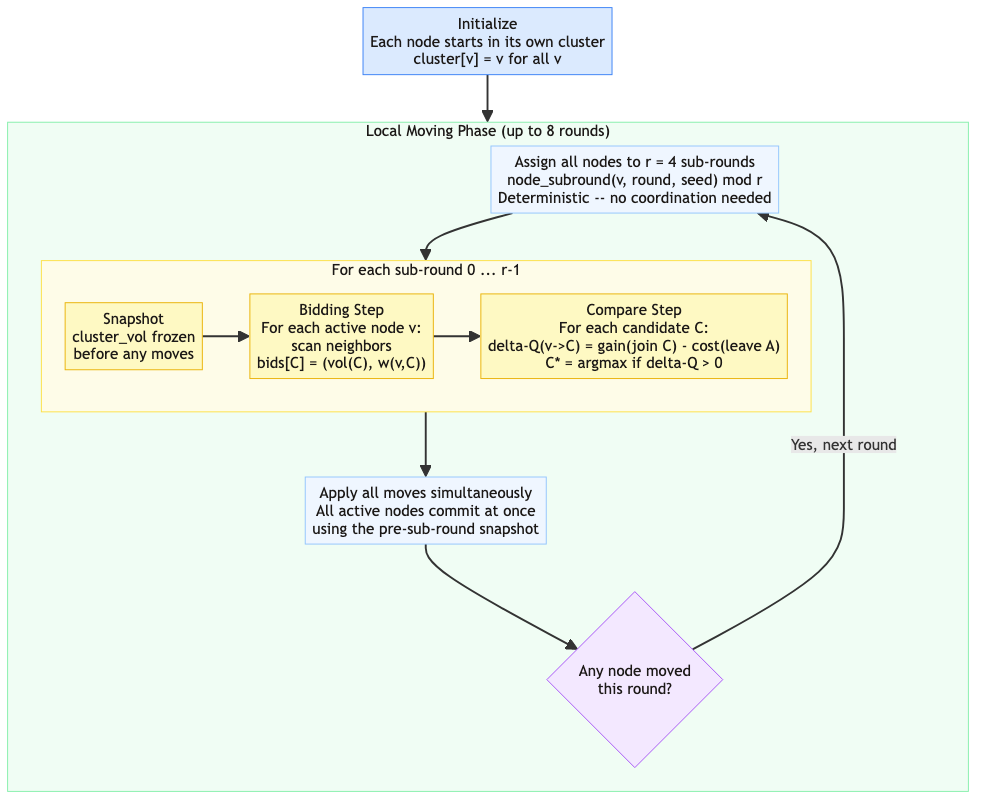
\includegraphics[height=0.82\textheight]{dslm_local_moving.png}
    \end{column}
    \begin{column}{0.46\textwidth}
      \textbf{Sub-round parallelization:}
      \begin{itemize}
        \item Hash assigns each node to one of 4 sub-rounds deterministically
        \item Cluster volumes are snapshotted before the sub-round begins
        \item All active nodes bid and commit simultaneously using the frozen snapshot
        \item Eliminates the sequential dependency that makes Louvain hard to parallelize
      \end{itemize}

      \bigskip
      Up to \textbf{8 rounds} per level before contraction.
    \end{column}
  \end{columns}
\end{frame}

% ===================================================================
% 5b. Algorithm Flow: Contraction and Unpacking
% ===================================================================
\begin{frame}{Algorithm Flow: Contraction and Unpacking}
  \begin{columns}[c]
    \begin{column}{0.50\textwidth}
      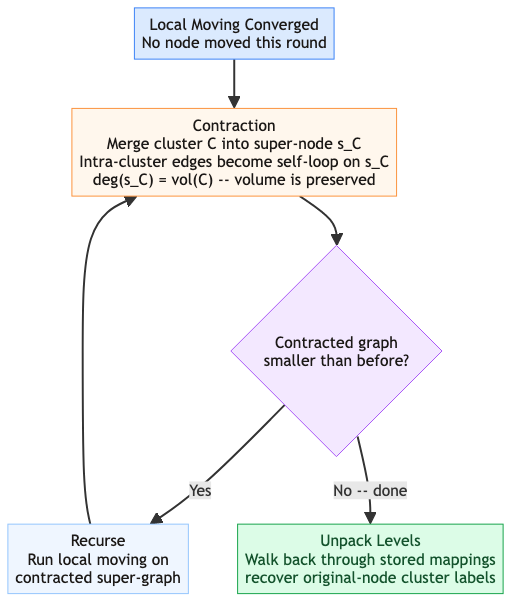
\includegraphics[height=0.78\textheight]{dslm_contraction.png}
    \end{column}
    \begin{column}{0.46\textwidth}
      \textbf{Why contraction matters:}
      \begin{itemize}
        \item Each cluster collapses into one super-node
        \item Graph shrinks dramatically: LiveJournal went from 4M nodes to 280K after level 0
        \item Self-loops must be preserved so super-node degree equals the original cluster volume
        \item Recurse until the graph stops shrinking, then unpack all levels
      \end{itemize}

      \bigskip
      Our run used \textbf{6 contraction levels} before converging.
    \end{column}
  \end{columns}
\end{frame}

% ===================================================================
% 6. Implementation
% ===================================================================
\begin{frame}{How I Coded It}
  \begin{columns}[c]
    \begin{column}{0.50\textwidth}
      \begin{center}
        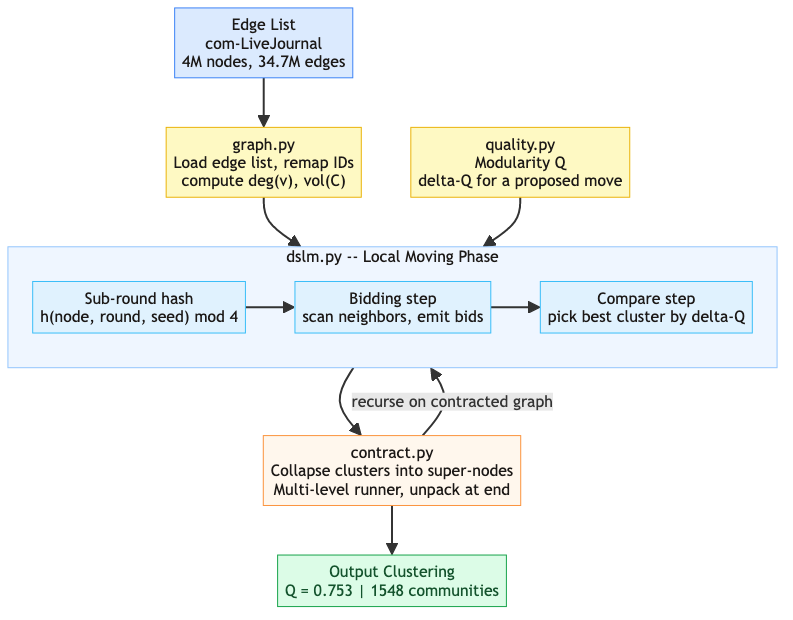
\includegraphics[height=0.80\textheight]{impl_flow.png}
      \end{center}
    \end{column}
    \begin{column}{0.46\textwidth}
      \textbf{Approach:} Sequential Python simulation that mirrors the distributed MapReduce data flow. No actual cluster needed.

      \bigskip
      \textbf{Key optimizations:}
      \begin{itemize}
        \item Fast CSV loading with pandas (52\,s vs.\ several minutes for naive row iteration)
        \item Incremental cluster volumes: update on each move instead of full recompute
      \end{itemize}
    \end{column}
  \end{columns}
\end{frame}

% ===================================================================
% 7. Results
% ===================================================================
\begin{frame}{Results vs. the Paper}
  \textbf{com-LiveJournal} (3.99M nodes, 34.7M edges)

  \medskip
  \begin{center}
  \begin{tabular}{lcc}
    \toprule
    Method & $Q$ & Time \\
    \midrule
    Louvain (paper)              & 0.713 & 99\,s \\
    PLM (paper)                  & 0.713 & 25\,s \\
    DSLM-Mod (paper)             & 0.710 & 31\,s \\
    DSLM-Mod w/o Cont.\ (paper)  & 0.622 & 14\,s \\
    \midrule
    NetworkX Louvain (ours)      & 0.746 & 7418\,s \\
    \textbf{Our DSLM-Mod (Python)} & \textbf{0.753} & 1119\,s \\
    \bottomrule
  \end{tabular}
  \end{center}

  \medskip
  \begin{itemize}
    \item $Q = 0.753$ beats all paper baselines; 6 contraction levels give a deeper search than a single pass
    \item Time gap reflects Python on one laptop vs.\ compiled C++ on a 32-host cluster, not algorithmic inefficiency
  \end{itemize}
\end{frame}

% ===================================================================
% 8. Conclusion
% ===================================================================
\begin{frame}{Conclusion}
  \begin{columns}[T]
    \begin{column}{0.48\textwidth}
      \textbf{What the paper contributes:}
      \begin{itemize}
        \item Sub-round hash breaks sequential dependency in local moving
        \item First distributed algorithm matching Louvain quality at scale
        \item Handles 100M+ nodes where GossipMap crashes or times out
        \item Up to 10$\times$ faster than prior distributed methods
      \end{itemize}
    \end{column}
    \begin{column}{0.48\textwidth}
      \textbf{What I found during implementation:}
      \begin{itemize}
        \item Self-loops during contraction are critical: dropping them collapses all clusters
        \item 8 rounds per level captures almost all quality ($+0.002$ for unlimited rounds, $5.8\times$ slower)
        \item Algorithm is easier to implement correctly than Louvain because the data flow is explicit
      \end{itemize}

      \bigskip
    \end{column}
  \end{columns}
\end{frame}

\end{document}
